\documentclass[12pt]{report}
\usepackage[a4paper, left=3.17cm, right=3.17cm, top=2.54cm, bottom=2.54cm]{geometry}
\usepackage[T1]{fontenc}
\usepackage{mathptmx}
\usepackage{amsmath}
\usepackage{amsfonts}
\usepackage{chemformula}
\usepackage{multicol}
\usepackage{multirow}
\usepackage{tabularx,booktabs}
\usepackage{array}
\usepackage{cite}
\usepackage{comment}
\usepackage{graphicx}
\usepackage{xcolor}
\usepackage{float}
\usepackage{listings}
\usepackage[linesnumbered,ruled,vlined]{algorithm2e}
\usepackage[colorlinks, linkcolor=black, anchorcolor=black, citecolor=black]{hyperref}
\newcolumntype{C}{>{\centering\arraybackslash}X}
\newcolumntype{P}[1]{>{\centering\arraybackslash}p{#1}}
\setlength{\parskip}{0.5em}
\title{Secure Data Transmission Application}

\lstdefinestyle{javacode}{
    language=Java,
    basicstyle=\ttfamily\small,
    keywordstyle=\color{blue},
    commentstyle=\color{teal},
    stringstyle=\color{red!70!black},
    numberstyle=\tiny\color{gray},
    numbers=left,
    numbersep=8pt,
    frame=single,
    breaklines=true,
    showstringspaces=false,
    tabsize=4
}
\lstset{style=javacode}

\usepackage{fancyhdr}
\fancyhf{}
\rfoot{%
  \footnotesize
  \textcopyright~Dept. of Computer Science and Engineering, GUB\\
}

\begin{document}
    \begin{titlepage}
\center
\newcommand{\HRule}{\rule{\linewidth}{0.1mm}}

\includegraphics[scale=0.6]{Figures/GUB.png}\\[1cm]
\center
\textsl{\Large Green University of Bangladesh }\\[0.5cm]
\textsl{\large Department of Computer Science and Engineering (CSE)}\\
\textsl{\large Semester: (Spring, Year: 2026), B.Sc. in CSE (Day)}\\[0.5cm]
\makeatletter
\HRule \\[0.4cm]
{ \huge \bfseries \@title}\\[0.2cm]
\HRule \\[1.0cm]

\textsl{\large Course Title: Data Communication Lab }\\
\textsl{\large Course Code: CSE 312 }\\
\textsl{\large Section: 241-D4}\\[0.5cm]

{\large \underline{Group Members}}\\[0.2cm]

\begin{table*}[htb]
\centering
\begin{tabular}{ |P{7.0cm}|P{3.5cm}|}
\hline
\textbf{Name} & \textbf{ID}\\
\hline
Md Kawsar Ahmed  & 222002131 \\
\hline
Ryan Hasan Sunny  & 213002183 \\
\hline
\end{tabular}
\end{table*}
\vspace{0.5cm}

\textsl{\large Submission Date: \ 10.04.2026 }\\
\textsl{\large Course Teacher's Name: \ Ms. Sagufta Sabah Nakshi }\\[0.9cm]

\makeatother
{\large [For teachers use only: \textcolor{red}{Don't write anything inside this box]}}\\

\begin{table}[]
\centering
\begin{tabular}{|p{7.5cm}p{7.0cm}|}
\hline
\multicolumn{2}{|c|}{{\underline{\textbf{Lab Project Status}}}} \\
 & \\\hline
\textbf{Marks:}                & \textbf{Signature:}        \\
 & \\
\textbf{Comments:}             & \textbf{Date:}             \\
 & \\\hline
\end{tabular}
\end{table}

\end{titlepage}

    \tableofcontents

\newpage
\chapter{Introduction}

\section{Overview}
Secure digital communication requires confidentiality, integrity, and a method of transmission that does not immediately attract suspicion. This project addresses that need by combining cryptography and image steganography in a single Java application. The developed system first encrypts a user message using a password-derived AES key and then hides the encrypted payload inside a digital image through least significant bit (LSB) substitution. The overall idea follows the standard motivation of steganographic systems: protect the meaning of the data through encryption while also concealing the existence of the data itself \cite{johnson1998exploring} \cite{fridrich2009steganography}.

The implemented application contains a graphical user interface for end users, a cryptographic module for password-based encryption and decryption, and an image-processing module for embedding and extracting hidden payloads. The final output is saved in PNG format so that the hidden bits are preserved. This design produces a practical secure data transmission workflow suitable for laboratory demonstration and small-scale confidential communication.

\section{Motivation}
The motivation behind this project can be summarized as follows:
\begin{itemize}
    \item Conventional plaintext transmission is insecure because intercepted messages can be read immediately.
    \item Encryption protects the message content, but it still reveals that secret communication is taking place.
    \item Steganography hides the existence of the message by placing it inside a normal looking digital image.
    \item Combining both approaches creates a stronger security model than using either one alone.
    \item The project is also a useful educational exercise in networking, image processing, GUI design, and applied cryptography.
\end{itemize}

\section{Problem Definition}

\subsection{Problem Statement}
The problem addressed in this work is how to transmit a confidential message through a common digital medium without exposing the message contents or revealing that hidden communication is taking place. A useful solution must satisfy four conditions:
\begin{itemize}
    \item The message must remain unreadable without the correct password.
    \item The carrier image must remain visually unchanged to human observers.
    \item The system must successfully recover the original message during decoding.
    \item The software must remain simple enough for students and nonexpert users to operate.
\end{itemize}

To solve this problem, the project implements a desktop application that encrypts a text message with a password and embeds the encrypted bytes into the RGB channels of a cover image using the LSB method.

\subsection{Complex Engineering Problem}
The developed system touches several attributes of a complex engineering problem. Table \ref{tab:IC} summarizes the main attributes addressed by this project.

\begin{table}[htbp]
   \centering
    \caption{Summary of the complex engineering attributes touched by the project}
    \begin{tabular}{|p{6.0 cm}|p{8 cm}|}
    \toprule
        \textbf{Name of the P Attributes} & \textbf{How the project addresses the attribute}  \\
        \midrule
    \textbf{P1:} Depth of knowledge required  & The project required knowledge of image representation, Java GUI development, password-based encryption, and byte-level data handling. \\
      \hline
    \textbf{P2:} Range of conflicting requirements  & The design balances security, hiding capacity, runtime efficiency, and ease of use. Higher security adds processing steps, while higher capacity increases image modification. \\
      \hline
    \textbf{P3:} Depth of analysis required  & The work required capacity analysis, payload framing, password validation, image format selection, and verification of message recovery. \\
    \hline
    \textbf{P4:} Familiarity of issues  & The project includes familiar issues such as incorrect passwords, unsupported images, insufficient capacity, and possible data corruption after lossy compression. \\
    \hline
    \textbf{P5:} Extent of applicable codes  & The implementation uses standard Java cryptographic libraries, image I/O libraries, and a custom LSB algorithm to meet secure transmission requirements. \\
      \hline
    \textbf{P6:} Extent of stakeholder involvement and conflicting requirements  & A usable interface was needed for normal users, while the internal design still had to satisfy technical security and data recovery constraints. \\
      \hline
    \textbf{P7:} Interdependence  & The GUI, encryption module, payload formatter, and image embedding module are tightly coupled; failure in one stage affects the complete transmission workflow. \\
    \hline
    \end{tabular}
    \label{tab:IC}
\end{table}

\section{Design Goals/Objectives}
The primary goal of the project was to develop a secure, user-friendly, and efficient message-hiding system. The design objectives are listed below.

\subsection{Security}
\textbf{Objective:} Protect the hidden message from unauthorized access.

\textbf{Methods Used:}
\begin{itemize}
    \item AES-GCM encryption with a 256-bit key derived from the user password.
    \item PBKDF2 key derivation with a random salt for each message.
    \item Password validation and authenticated decryption to detect invalid credentials or tampered payloads.
\end{itemize}

\subsection{Usability}
\textbf{Objective:} Make the system easy to use through a desktop interface.

\textbf{Methods Used:}
\begin{itemize}
    \item Swing-based graphical interface with separate tabs for encoding and decoding.
    \item File selection dialogs for choosing input and output images.
    \item Clear feedback for successful embedding, extraction, capacity checks, and error conditions.
\end{itemize}

\subsection{Efficiency}
\textbf{Objective:} Embed and recover messages without noticeable delay or visible image degradation.

\textbf{Methods Used:}
\begin{itemize}
    \item Direct manipulation of image RGB channels through Java buffered images.
    \item Payload framing that stores only the necessary metadata.
    \item PNG output to preserve embedded bits without repeated quality loss.
\end{itemize}

\section{Application}
The project can be used in several practical scenarios:
\begin{itemize}
    \item \textbf{Secure messaging:} Short confidential text can be sent inside harmless looking images.
    \item \textbf{Academic demonstration:} The application is suitable for teaching encryption, steganography, and digital image processing.
    \item \textbf{Digital watermarking concepts:} The same embedding idea can be extended to store ownership or integrity information.
    \item \textbf{Confidential lab communication:} A message can be exchanged without exposing its presence in ordinary file sharing environments.
\end{itemize}

\newpage
\chapter{Design/Development/Implementation of the Project}

\section{Introduction}
This chapter explains how the Secure Data Transmission Application was designed and implemented. The final system is a layered desktop application written in Java 17. Its main workflow is simple: the user chooses an image, writes a secret message, enters a password, and saves a new PNG image. Internally, the message is converted into ciphertext using modern symmetric encryption and then inserted into the least significant bits of image pixels. During recovery, the application extracts the hidden payload, reconstructs the encrypted block, and decrypts it using the same password. This dual-protection model is consistent with the established role of steganography and cryptography in secure information hiding \cite{fridrich2009steganography} \cite{stallings2017cryptography}.

\section{Project Details}

\subsection{System Architecture}
The project was implemented as four cooperating layers:
\begin{itemize}
    \item \textbf{User interface layer:} Swing forms for encode and decode operations.
    \item \textbf{Cryptography layer:} Password validation, key derivation, AES-GCM encryption, and AES-GCM decryption.
    \item \textbf{Payload layer:} Formatting of salt, IV, version marker, and ciphertext into a recoverable byte structure.
    \item \textbf{Steganography layer:} LSB insertion into RGB channels and extraction from the stego image.
\end{itemize}

Figure \ref{fig:workflow} shows the complete workflow used by the application.

\begin{figure}[H]
    \centering
    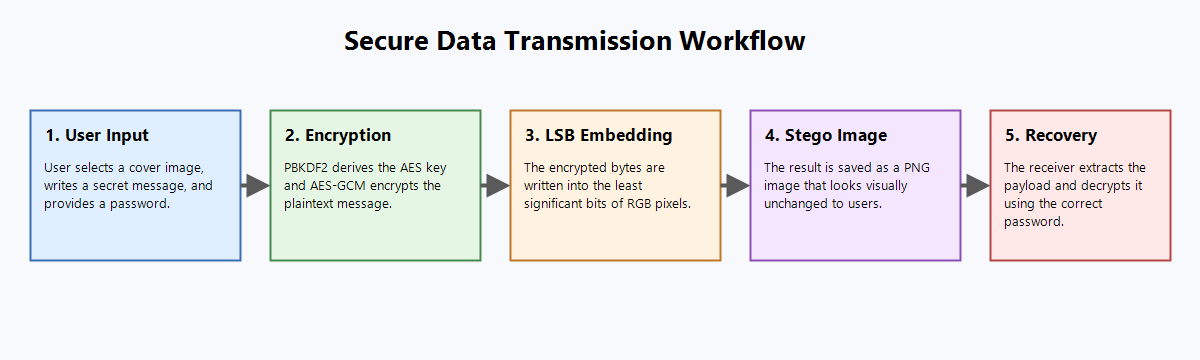
\includegraphics[width=\textwidth]{Figures/system_workflow.png}
    \caption{Overall workflow of the Secure Data Transmission Application}
    \label{fig:workflow}
\end{figure}

\subsection{Internal Data Format}
The embedded payload is not just raw ciphertext. A fixed structure was used so the program can safely identify and recover the hidden data:
\begin{itemize}
    \item A four-byte magic header to identify a valid payload.
    \item A one-byte version field for future compatibility.
    \item A 16-byte random salt for PBKDF2.
    \item A 12-byte initialization vector for AES-GCM.
    \item A four-byte ciphertext length.
    \item The ciphertext itself.
\end{itemize}

This structure prevents the decoder from treating arbitrary image noise as a valid message.

\subsection{Project Files}
The major files created in the complete project are:
\begin{itemize}
    \item \texttt{src/com/securetransmission/AppLauncher.java}
    \item \texttt{src/com/securetransmission/ui/MainFrame.java}
    \item \texttt{src/com/securetransmission/core/CryptoUtils.java}
    \item \texttt{src/com/securetransmission/core/SteganographyService.java}
    \item \texttt{src/com/securetransmission/cli/StegoCli.java}
    \item \texttt{scripts/compile.ps1}, \texttt{scripts/run-gui.ps1}, and \texttt{scripts/run-cli.ps1}
\end{itemize}

\section{Implementation}
This section describes the actual implementation of the software in detail.

\subsection{Development Environment}
The project was implemented and tested with the environment shown in Table \ref{tab:tools}.

\begin{table}[H]
    \centering
    \caption{Tools and libraries used in the project}
    \label{tab:tools}
    \begin{tabularx}{\textwidth}{|p{4.2cm}|X|}
        \hline
        \textbf{Component} & \textbf{Usage in the project} \\
        \hline
        Java 17 & Primary programming language and runtime environment \\
        \hline
        Swing & Desktop graphical user interface \\
        \hline
        javax.crypto & AES-GCM encryption and decryption \\
        \hline
        PBKDF2WithHmacSHA256 & Password-based 256-bit key derivation \\
        \hline
        BufferedImage / ImageIO & Loading, editing, and saving image files \\
        \hline
        PowerShell scripts & Build, run, and command-line testing automation \\
        \hline
    \end{tabularx}
\end{table}

\subsection{The Workflow}
The complete encoding workflow implemented in the application is:
\begin{enumerate}
    \item Read the cover image selected by the user.
    \item Accept the secret text and password from the interface.
    \item Generate a random salt and IV.
    \item Derive a 256-bit AES key from the password using PBKDF2.
    \item Encrypt the plaintext message with AES-GCM.
    \item Build a structured payload containing header, salt, IV, length, and ciphertext.
    \item Check whether the cover image has enough embedding capacity.
    \item Store the payload bits inside the least significant bits of RGB channels.
    \item Save the result as a PNG stego image.
\end{enumerate}

The decoding workflow performs the reverse sequence:
\begin{enumerate}
    \item Read the selected stego image.
    \item Extract the payload length from the first four bytes.
    \item Recover the remaining framed payload.
    \item Validate the magic header and payload version.
    \item Rebuild the encrypted packet from the embedded bytes.
    \item Derive the AES key from the provided password.
    \item Decrypt the message and display it to the user.
\end{enumerate}

\subsection{Encoding and Decoding Workflow Screenshots}
For report presentation, only two screenshots are used to summarize the complete working procedure of the application. The first screenshot shows the encoding interface after selecting the cover image, entering the password, and typing the secret message. The second screenshot shows the decoding interface after loading the stego image and recovering the original plaintext.

\begin{figure}[H]
    \centering
    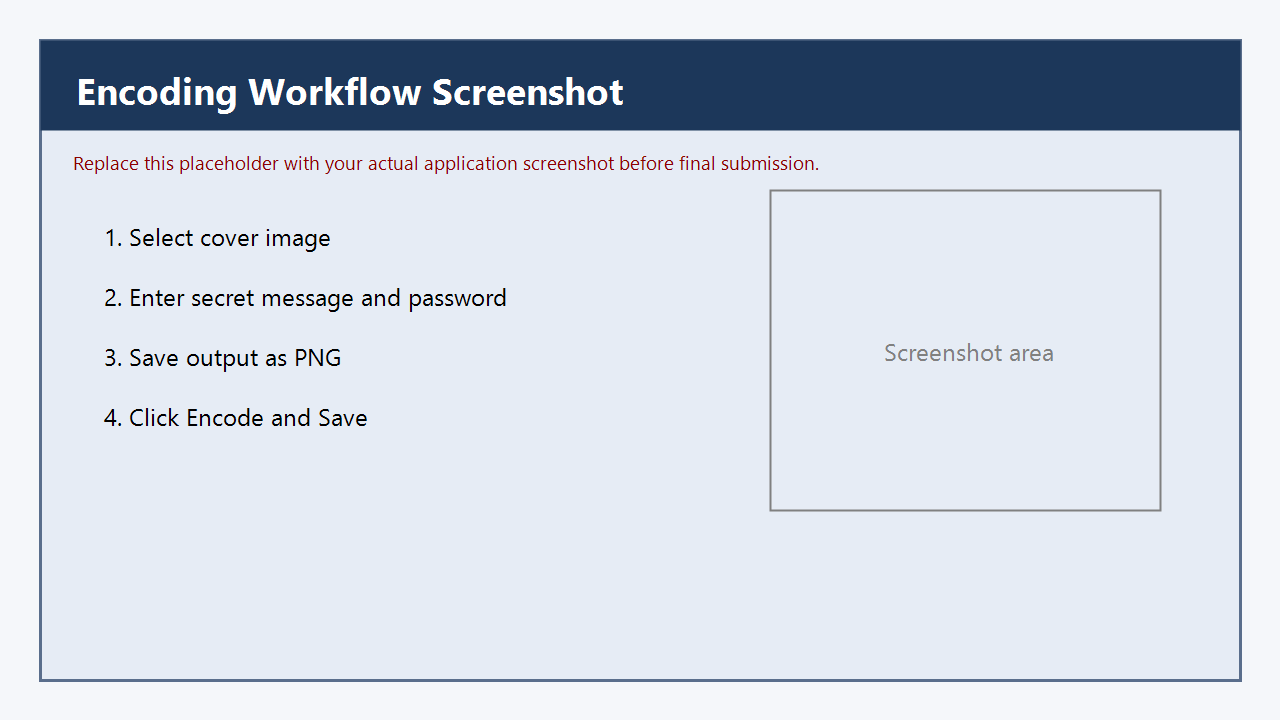
\includegraphics[width=0.92\textwidth]{Figures/encode_workflow.png}
    \caption{Encoding workflow of the application}
    \label{fig:encode-workflow}
\end{figure}

\begin{figure}[H]
    \centering
    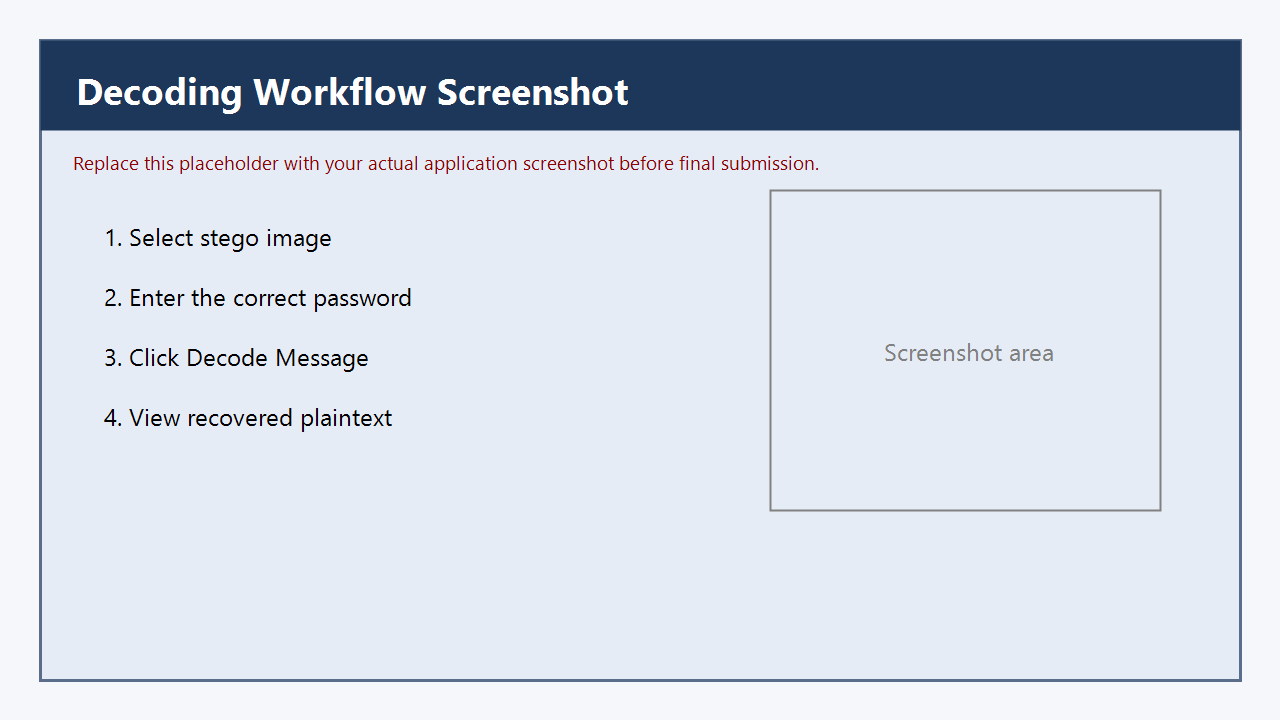
\includegraphics[width=0.92\textwidth]{Figures/decode_workflow.png}
    \caption{Decoding workflow of the application}
    \label{fig:decode-workflow}
\end{figure}

\subsection{Implementation Details}

\subsubsection{Encryption Module}
The cryptographic module is implemented in \texttt{CryptoUtils.java}. A password with at least eight characters is required. The program uses a random 16-byte salt and a 12-byte IV for every encoding operation. PBKDF2WithHmacSHA256 derives a 256-bit key from the password, and AES/GCM/NoPadding performs authenticated encryption. GCM mode is suitable here because it provides confidentiality and also detects tampering during decryption \cite{stallings2017cryptography}.

\begin{lstlisting}[caption={Core AES-GCM encryption logic used in the project}]
byte[] salt = new byte[16];
byte[] iv = new byte[12];
SECURE_RANDOM.nextBytes(salt);
SECURE_RANDOM.nextBytes(iv);

PBEKeySpec keySpec = new PBEKeySpec(password, salt, 65536, 256);
SecretKeyFactory factory = SecretKeyFactory.getInstance("PBKDF2WithHmacSHA256");
byte[] keyBytes = factory.generateSecret(keySpec).getEncoded();
SecretKey secretKey = new SecretKeySpec(keyBytes, "AES");

Cipher cipher = Cipher.getInstance("AES/GCM/NoPadding");
cipher.init(Cipher.ENCRYPT_MODE, secretKey, new GCMParameterSpec(128, iv));
byte[] cipherText = cipher.doFinal(plainText.getBytes(StandardCharsets.UTF_8));
\end{lstlisting}

\subsubsection{Steganography Module}
The steganography engine is implemented in \texttt{SteganographyService.java}. Each pixel contributes three storage bits: one from the red channel, one from the green channel, and one from the blue channel. The alpha channel is left unchanged. Since only the least significant bits are modified, the visual effect remains extremely small.

\begin{lstlisting}[caption={LSB embedding logic used in the project}]
if (bitIndex < totalBits) {
    red = (red & 0xFE) | getBit(data, bitIndex++);
}
if (bitIndex < totalBits) {
    green = (green & 0xFE) | getBit(data, bitIndex++);
}
if (bitIndex < totalBits) {
    blue = (blue & 0xFE) | getBit(data, bitIndex++);
}

int updatedArgb = (alpha << 24) | (red << 16) | (green << 8) | blue;
image.setRGB(x, y, updatedArgb);
\end{lstlisting}

\subsubsection{Graphical User Interface}
The user interface is implemented in \texttt{MainFrame.java}. It contains two tabs:
\begin{itemize}
    \item \textbf{Encode tab:} Input image selection, output image selection, password field, message field, capacity checking, and encode action.
    \item \textbf{Decode tab:} Stego image selection, password input, and recovered message display.
\end{itemize}

This layout keeps the software easy to operate while still exposing the full secure transmission workflow.

\subsubsection{Error Handling}
The application validates common failure cases before or during execution:
\begin{itemize}
    \item Empty message input
    \item Password shorter than eight characters
    \item Missing or unsupported image file
    \item Insufficient image capacity
    \item Invalid hidden payload
    \item Incorrect password during extraction
\end{itemize}

\section{Algorithms}
The two most important algorithms are the embedding algorithm and the extraction algorithm.

\begin{algorithm}[H]
\DontPrintSemicolon
\KwInput{Cover image $I$, plaintext message $M$, password $P$}
\KwOutput{Stego image $S$}
Generate random salt and IV\;
Derive AES key from $P$ using PBKDF2\;
Encrypt $M$ with AES-GCM to produce ciphertext $C$\;
Build payload $D = [magic, version, salt, IV, len(C), C]$\;
Store payload length before $D$\;
Check whether $I$ has enough RGB-LSB capacity\;
\ForEach{pixel in the image}
{
    Replace the LSB of red, green, and blue with the next payload bits\;
    \If{all bits are embedded}
    {
        stop embedding\;
    }
}
Save the modified image as PNG\;
\caption{Encoding algorithm}
\end{algorithm}

\begin{algorithm}[H]
\DontPrintSemicolon
\KwInput{Stego image $S$, password $P$}
\KwOutput{Recovered plaintext message $M$}
Read the first four embedded bytes to obtain the payload length\;
Extract the complete framed payload from RGB-LSB positions\;
Verify the magic header and payload version\;
Recover salt, IV, and ciphertext from the payload\;
Derive the AES key from $P$ using PBKDF2\;
Decrypt the ciphertext using AES-GCM\;
\If{decryption succeeds}
{
    Return the original plaintext message\;
}
\Else
{
    Report invalid password or damaged payload\;
}
\caption{Decoding algorithm}
\end{algorithm}

\newpage
\chapter{Performance Evaluation}

\section{Simulation Environment/Simulation Procedure}
The project was tested on a Windows environment with Java 17 installed. The source code was compiled through PowerShell scripts, and the application was validated with both the graphical interface and the CLI. The main test procedure was:
\begin{enumerate}
    \item Compile the source files into the \texttt{out} directory.
    \item Measure the available payload capacity of the sample PNG image.
    \item Encode a sample text message into the image.
    \item Decode the hidden text using the correct password.
    \item Attempt extraction with an incorrect password.
    \item Compare the original and stego images to count changed pixels and channels.
\end{enumerate}

\subsection{Sample Test Case}
The demonstration used \texttt{Figures/CEP.png} as the cover image. The sample message contained 161 UTF-8 bytes, and the generated stego output was saved as \texttt{Figures/stego\_sample.png}.

\section{Results Analysis/Testing}

\subsection{Functional Verification}
Table \ref{tab:functional-results} summarizes the core functional test results.

\begin{table}[H]
    \centering
    \caption{Functional verification results}
    \label{tab:functional-results}
    \begin{tabularx}{\textwidth}{|p{5cm}|X|p{2.5cm}|}
        \hline
        \textbf{Test item} & \textbf{Observed behavior} & \textbf{Result} \\
        \hline
        Capacity check & The CLI reported an available payload capacity of 156160 bytes for the selected PNG image. & Passed \\
        \hline
        Encoding with valid password & The message was embedded successfully and the stego image was saved without runtime errors. & Passed \\
        \hline
        Decoding with correct password & The application recovered the original plaintext message exactly. & Passed \\
        \hline
        Decoding with incorrect password & The application rejected the operation with an authentication/decryption error. & Passed \\
        \hline
    \end{tabularx}
\end{table}

\subsection{Image Quality and Capacity Analysis}
Table \ref{tab:metrics} presents measured values from the implemented system.

\begin{table}[H]
    \centering
    \caption{Measured project metrics from the sample run}
    \label{tab:metrics}
    \begin{tabularx}{\textwidth}{|p{6cm}|X|}
        \hline
        \textbf{Metric} & \textbf{Measured value} \\
        \hline
        Cover image resolution & 823 $\times$ 506 pixels \\
        \hline
        Cover image file size & 95551 bytes \\
        \hline
        Stego image file size & 85916 bytes \\
        \hline
        Available payload capacity & 156160 bytes \\
        \hline
        Secret message length & 161 bytes \\
        \hline
        Changed pixels after embedding & 508 pixels \\
        \hline
        Percentage of changed pixels & 0.122\% of the image pixels \\
        \hline
        Changed RGB channels & 896 channels \\
        \hline
        Percentage of changed RGB channels & 0.0717\% of all RGB channel values \\
        \hline
    \end{tabularx}
\end{table}

The results show that only a very small portion of pixels needed modification to hide the encrypted message. Since each channel changes by at most one bit, the visual difference between the original and stego image remains negligible.

\subsection{Visual Comparison}
Figure \ref{fig:stego-comparison} shows the original sample image and the generated stego image used during testing.

\begin{figure}[H]
    \centering
    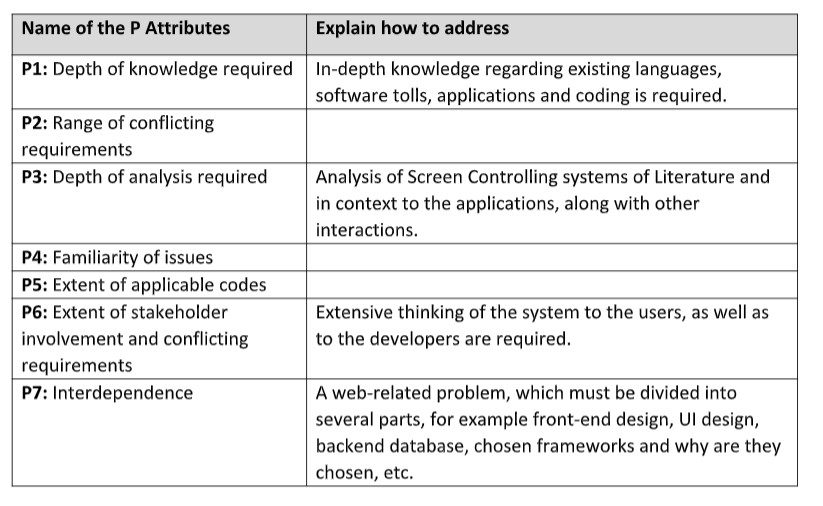
\includegraphics[width=0.45\textwidth]{Figures/CEP.png}
    \hfill
    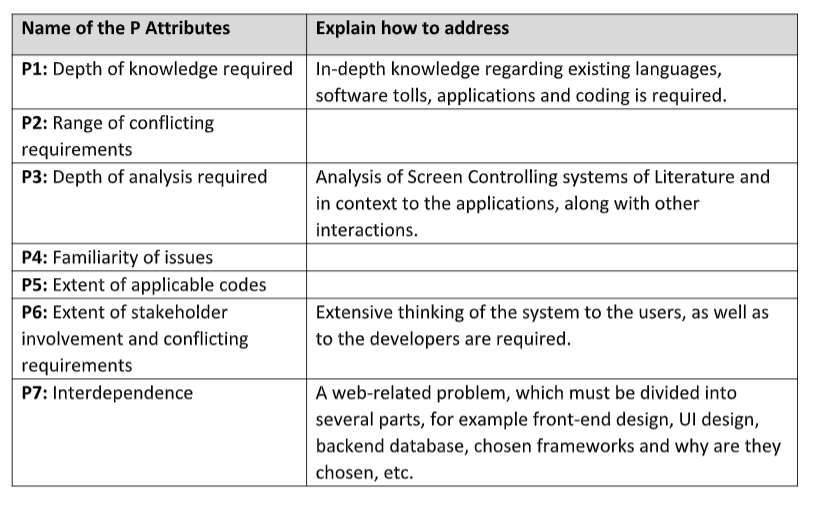
\includegraphics[width=0.45\textwidth]{Figures/stego_sample.png}
    \caption{Left: original cover image. Right: stego image containing the encrypted message.}
    \label{fig:stego-comparison}
\end{figure}

\section{Results Overall Discussion}
The performance evaluation confirms that the system meets the stated design objectives. The program can successfully encrypt, embed, extract, and decrypt short text messages using a password-driven workflow. The measured pixel-change percentages are very low, which supports the claim that LSB substitution maintains good visual transparency for modest message sizes. The use of AES-GCM also improves system reliability because a wrong password or tampered payload triggers decryption failure instead of producing misleading output.

\subsection{Complex Engineering Problem Discussion}
The results demonstrate how multiple engineering concerns interact in a single application. Security requirements affected key derivation, payload design, and validation logic. Image-processing decisions affected capacity and transparency. User-interface choices affected accessibility and error prevention. The final application therefore reflects the interdependence and design tradeoffs described earlier in Table \ref{tab:IC}.

\newpage
\chapter{Conclusion}

\section{Discussion}
This project successfully developed a complete Secure Data Transmission Application that combines password-based AES encryption with image steganography. The implemented Java application includes a GUI for ordinary users, a CLI for testing, a structured payload format, and image-based hiding using RGB LSB substitution. Experimental results confirmed that the hidden message can be recovered correctly with the proper password while incorrect credentials are rejected.

\section{Limitations}
Despite the successful implementation, the project has some practical limitations:
\begin{itemize}
    \item The application is intended for text messages only and does not yet support arbitrary file embedding.
    \item The current embedding method uses simple sequential LSB substitution, which is easy to understand but not the most resistant to advanced steganalysis.
    \item The hidden payload is vulnerable if the final image is converted into a lossy format such as JPEG.
    \item The project focuses on desktop execution and does not yet provide network-based sender and receiver synchronization.
\end{itemize}

\section{Scope of Future Work}
Several useful improvements can be added in future work:
\begin{itemize}
    \item Support for hiding documents or binary files in addition to text.
    \item More advanced embedding strategies such as randomized pixel selection or edge-based hiding.
    \item Automatic image quality metrics such as PSNR and SSIM after embedding.
    \item A sender-receiver communication module for direct secure file transfer.
    \item Cross-platform packaging and database logging for message history.
\end{itemize}

\newpage
\renewcommand\bibname{References}
\bibliographystyle{unsrt}
\bibliography{Ref}

\end{document}
